\section{Materia Heterogénea}\label{sec:heterogeneous}

	La clase `Heterogeneous' se encarga de los cálculos de equilibrio entre las fases líquido y vapor. La clase contiene dos objetos del tipo `Homogeneous' que representan a la fase líquida y a la fase vapor. La clase implementa los algoritmos numéricos para igualar los cálculos de la fugacidad entre las fases.

	Los cálculos de equilibrio que se implementan en este trabajo son:

	\begin{itemize}\itemsep0ex

		\item Substancias
			\begin{itemize}\itemsep0ex
				\item Temperatura de saturación.\ref{subsec:saturationtemperature}
				\item Presión de saturación.\ref{subsec:saturationpressure}
			\end{itemize}

		\item Mezclas
	\begin{itemize}\itemsep0ex
		\item Presión de burbuja, sección \ref{subsec:bubblepressure}.
		\item Presión de rocío, sección \ref{subsec:dewpressure}.
		\item Temperatura de burbuja, sección \ref{subsec:bubbletemperature}.
		\item Temperatura de rocío, sección \ref{subsec:dewtemperature}.
		\item Flash temperatura-presión \ref{subsec:flash}.
	\end{itemize}

	\end{itemize}

	Los algoritmos son muy similares, las principales diferencias consisten en la función objetivo.

	La clase `HeterogeneousSubstance' realiza los cálculos de equilibrio para las substancias y la clase `HeterogeneousMixture' realiza los cálculos de equilibrio para las mezclas, en la figura \ref{fig:heterogeneous} se muestra la estructura.

\begin{figure}[!h]
  \centering
    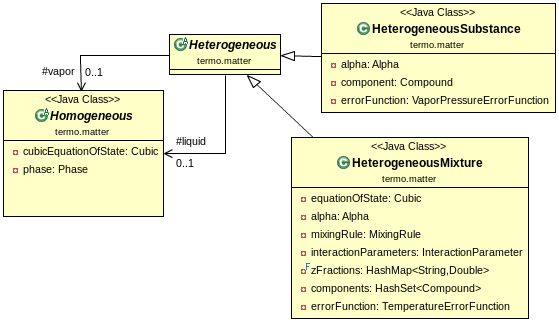
\includegraphics[scale=0.7]{heterogeneous.png}
    \caption{Estructura de la librería para el cálculo de equilibrio Líquido-Vapor.}
    \label{fig:heterogeneous}
\end{figure}

	Los cálculos de la presente sección se realizan de forma muy similar, primero indicando la variable conocida con el método `set', después invocando el método que realiza el algoritmo para conocer la incognita (el método puede recibir o no un estimado inicial) y finalmente obtener el resultado de la variable con el método `get'.

	Cada sección muestra el uso de la librería con fragmentos de código que realizan el cálculo con y sin el estimado inicial. También se indica el método empleado para estimar la varible incognita en caso de no proporcionar un estimado inicial.

	Todos los diagramas de los algoritmos se muestran en el apéndice \ref{chap:algorithms}.

	La librería \Materia intenta evitar usar clases que no tengan relación con conceptos de termodinámica o de ingeniería química, sin embargo para los siguientes métodos es necesario utilizar otro tipo de clase para indicar los estimados de las fracciones molares de las mezclas. Para indicar las fracciones mol de cada compuesto se utiliza el objeto 'Map<String,Double>' que relaciona el nombre del compuesto con el valor de la fracción molar. Típicamente el estimado de las fracciones se debe guardar entre cambios de temperatura o presión en cálculos de rocío o de burbuja, para evitar la divergencia de los métodos numéricos al acercarse a la región del punto crítico. Para guardar las fracciones molares de una mezcla homogénea se utilza el método 'getFractions()' que devuelve un objeto del tipo 'Map<String,Double>'. Esta clase solo es necesaria para los cálculos en mezclas heterogéneas. El código \ref{lst:estimatedFractions} muestra como guardar las fracciones del líquido o del vapor para ser usadas como estimados iniciales de los próximos cálculos de equilibrio.


	\begin{lstlisting}[caption={Para guardar las fracciones molares del líquido o del vapor en un objeto del tipo 'Map$<$String,Double$>$' que se usará en los métodos de presión y temperatura de equilibrio} ,label={lst:estimatedFractions}]
		Map<String,Double> liquidFractions = 
					heterogeneousMixture.getLiquid().getFractions();

		Map<String,Double> vaporFractions = 
					heterogeneousMixture.getVapor().getFractions();
		
	\end{lstlisting}

		
\subsection{Temperatura de saturación}\label{subsec:saturationtemperature}


	El cálculo de temperatura de saturación se realiza como se indica en la figura \ref{fig:saturationtemperature}. Usando un objeto del tipo `HeterogeneousSubstance' de la librería \Materia el cálculo se realiza como se muestra en los fragmentos de código \ref{lst:saturationtemperature} y \ref{lst:saturationtemperatureWithEstimate}.

	Si al método no se le proporciona un estimado inicial, como se muestra en el código \ref{lst:saturationtemperature} entonces la clase realiza la estimación como se muestra en el diagrama \ref{fig:temperatureEstimate}. 

	

	\begin{lstlisting}[label={lst:saturationtemperatureWithEstimate},caption={Cálculo de la temperatura de saturación proporcionando un estimado inicial.}]
		heterogeneousSubstance.setPressure(pressure);
		heterogeneousSubstance.saturationTemperature(temperatureEstimate);
		double temperature = heterogeneousSubstance.getTemperature();
	\end{lstlisting}


	\begin{lstlisting}[label={lst:saturationtemperature},caption={Cálculo de la temperatura de saturación.}]
		heterogeneousSubstance.setPressure(pressure);
		heterogeneousSubstance.saturationTemperature();
		double temperature = heterogeneousSubstance.getTemperature();
	\end{lstlisting}

	%hecho
\subsection{Presión de saturación}\label{subsec:saturationpressure}

	El cálculo de presión de saturación se realiza como se indica en la figura \ref{fig:saturationpressure}. Usando un objeto del tipo `HeterogeneousSubstance' de la librería \Materia el cálculo se realiza como se muestra en los fragmentos de código \ref{lst:saturationpressure} y \ref{lst:saturationpressureWithEstimate}.

	Si al método no se le proporciona un estimado inicial, como se muestra en el código \ref{lst:saturationpressure} entonces la clase realiza la estimación de la presión de vapor con la ecuación del factor acéntrico \ref{eq:pressureacentricfactor}. 

	\begin{lstlisting}[label={lst:saturationpressureWithEstimate},caption={Cálculo de la presión de saturación proporcionando un estimado inicial.}]
		heterogeneousSubstance.setTemperature(temperature);
		heterogeneousSubstance.saturationPressure(pressureEstimate);
		double pressure = heterogeneousSubstance.getPressure();
	\end{lstlisting}


	\begin{lstlisting}[label={lst:saturationpressure},caption={Cálculo de la presión de saturación.}]
		heterogeneousSubstance.setTemperature(temperature);
		heterogeneousSubstance.saturationPressure();
		double pressure = heterogeneousSubstance.getPressure();
	\end{lstlisting}

	Las figuras \ref{fig:saturationPressure} y \ref{fig:saturationPressure3d} muestran el resultado del cálculo de la presión de saturación para el agua con la ecuación de estado de Peng Robinson.

\begin{figure}[!h]
	\centering	
	\begin{tikzpicture}
	\begin{axis}[xlabel=\temperature,ylabel=\pressure]
	\addplot[blue,smooth]table{plotdata/heterogeneous/et.dat};
	\end{axis}
	\end{tikzpicture}
	\caption{Diagrama de presión de saturación para el agua con la ecuación de estado de Peng Robinson}\label{fig:saturationPressure}
\end{figure}

\begin{figure}[!h]
	\centering
	\begin{tikzpicture}
	\begin{axis}[view/h=-165,xlabel={\temperature},ylabel={\molarVolume},zlabel=\pressure,colorbar,
					colorbar style={ylabel=Temperatura (K),
					 							title=Código de color}]
	\addplot3[surf,point meta=explicit]table[meta=temperature, x=temperature , y=liquidVolume, z=pressure]{plotdata/heterogeneous/et.dat};
	\addplot3[surf,point meta=explicit]table[meta=temperature, x=temperature , y=vaporVolume, z=pressure]{plotdata/heterogeneous/et.dat};
	\end{axis}
	\end{tikzpicture}
	\caption{Diagrama tridimensional de presión de saturación - temperatura- volumen molar para el agua con la ecuación de estado de Peng Robinson}
	\label{fig:saturationPressure3d}
\end{figure}%hecho

\subsection{Temperatura de Burbuja}\label{subsec:bubbletemperature}

	El cálculo de temperatura de burbuja para una mezcla se realiza como se indica en la figura \ref{fig:bubbletemperature}. Usando un objeto del tipo `HeterogeneousMixture' de la librería \Materia el cálculo se realiza como se muestra en los fragmentos de código \ref{lst:bubbletemperature} y \ref{lst:bubbletemperatureWithEstimate}.

	Si al método no se le proporciona un estimado inicial, como se muestra en el código \ref{lst:bubbletemperature} entonces la clase realiza la estimación de la temperatura como se muestra en la figura \ref{fig:bubbletemperatureEstimate}. 

	\begin{lstlisting}[label={lst:bubbletemperatureWithEstimate},caption={Cálculo de la temperatura de burbuja proporcionando un estimado inicial.}]

		heterogeneousMixture.setZFraction(compound1,molarFraction1);
		//...... asignar la fracción molar para todos los compuestos

		heterogeneousMixture.setPressure(pressure);
		heterogeneousMixture.bubbleTemperature(temeperatureEstimate);
		double temperature = heterogeneousMixture.getTemperature();
	\end{lstlisting}


	\begin{lstlisting}[label={lst:bubbletemperature},caption={Cálculo de la temperatura de burbuja.}]

		heterogeneousMixture.setZFraction(compound1,molarFraction1);
		//...... asignar la fracción molar para todos los compuestos

		heterogeneousMixture.setPressure(pressure);
		heterogeneousMixture.bubbleTemperature();
		double temperature = heterogeneousMixture.getTemperature();
	\end{lstlisting}


%hecho
\subsection{Temperatura de Rocío}\label{subsec:dewtemperature}

	El cálculo de temperatura de rocío para una mezcla se realiza como se indica en la figura \ref{fig:dewtemperature}. Usando un objeto del tipo `HeterogeneousMixture' de la librería \Materia el cálculo se realiza como se muestra en los fragmentos de código \ref{lst:dewtemperature} y \ref{lst:dewtemperatureWithEstimate}.

	Si al método no se le proporciona un estimado inicial, como se muestra en el código \ref{lst:dewtemperature} entonces la clase realiza la estimación de la temperatura como se muestra en la figura \ref{fig:dewtemperatureEstimate}. 

	\begin{lstlisting}[label={lst:dewtemperatureWithEstimate},caption={Cálculo de la temperatura de rocío proporcionando un estimado inicial.}]

		heterogeneousMixture.setZFraction(compound1,molarFraction1);
		//...... asignar la fracción molar para todos los compuestos

		heterogeneousMixture.setPressure(pressure);
		heterogeneousMixture.dewTemperature(
			temeperatureEstimate,liquidEstimatedFractions);
		double temperature = heterogeneousMixture.getTemperature();
	\end{lstlisting}


	\begin{lstlisting}[label={lst:dewtemperature},caption={Cálculo de la temperatura de rocío.}]

		heterogeneousMixture.setZFraction(compound1,molarFraction1);
		//...... asignar la fracción molar para todos los compuestos

		heterogeneousMixture.setPressure(pressure);
		heterogeneousMixture.dewTemperature();
		double temperature = heterogeneousMixture.getTemperature();
	\end{lstlisting}

%hecho
\subsection{Presión de Burbuja}\label{subsec:bubblepressure}

	El cálculo de presión de burbuja para una mezcla se realiza como se indica en la figura \ref{fig:bubblepressure}. Usando un objeto del tipo `HeterogeneousMixture' de la librería \Materia el cálculo se realiza como se muestra en los fragmentos de código \ref{lst:bubblepressure} y \ref{lst:bubblepressureWithEstimate}.

	Si al método no se le proporciona un estimado inicial, como se muestra en el código \ref{lst:bubblepressure} entonces la clase realiza la estimación de la presión de vapor con la ecuación del factor acéntrico \ref{eq:pressureacentricfactor}. 



	\begin{lstlisting}[label={lst:bubblepressureWithEstimate},caption={Cálculo de la presión de burbuja proporcionando un estimado inicial.}]

		heterogeneousMixture.setZFraction(compound1,molarFraction1);
		//...... asignar la fracción molar para todos los compuestos

		heterogeneousMixture.setTemperature(temperature);
		heterogeneousMixture.bubblePressure(pressureEstimate);
		double pressure = heterogeneousMixture.getPressure();
	\end{lstlisting}


	\begin{lstlisting}[label={lst:bubblepressure},caption={Cálculo de la presión de burbuja.}]
		heterogeneousMixture.setZFraction(compound1,molarFraction1);
		//...... asignar la fracción molar para todos los compuestos

		heterogeneousMixture.setTemperature(temperature);
		heterogeneousMixture.bubblePressure();
		double pressure = heterogeneousMixture.getPressure();
	\end{lstlisting}

	La figura \ref{fig:bubblepressure3d} muestra el resultado del cálculo de presión de burbuja para el sistema metanol-agua.

\begin{figure}[p]
\centering
	\begin{tikzpicture}
	\begin{axis}[view/v=-15,colorbar left,xlabel={Fracción Molar del metanol},ylabel=\temperature,zlabel=\pressure,colorbar style={ylabel=\temperature,
        yticklabel style={
            text width=2.5em,
            align=right}}]
		\addplot3[surf,point meta=explicit,shader=interp]table[meta=temperature, y=temperature , x=liquidFraction, z=pressure]{plotdata/mixhet/hp.dat};
		\addplot3[surf,point meta=explicit,shader=interp]table[meta=temperature, y=temperature , x=vaporFraction, z=pressure]{plotdata/mixhet/hp.dat};
	\end{axis}
	\end{tikzpicture}


	\begin{tikzpicture}
	\begin{axis}[view/v=-220,xlabel={Fracción Molar del metanol},ylabel=\temperature,zlabel=\pressure]
	\addplot3[surf,point meta=explicit,shader=interp]table[meta=temperature, y=temperature , x=liquidFraction, z=pressure]{plotdata/mixhet/hp.dat};
	\addplot3[surf,point meta=explicit,shader=interp]table[meta=temperature, y=temperature , x=vaporFraction, z=pressure]{plotdata/mixhet/hp.dat};
	\end{axis}
	\end{tikzpicture}


	\begin{tikzpicture}
	\begin{axis}[view/v=-115,xlabel={Fracción Molar del metanol},ylabel=\temperature,zlabel=\pressure]
	\addplot3[surf,point meta=explicit,shader=interp]table[meta=temperature, y=temperature , x=liquidFraction, z=pressure]{plotdata/mixhet/hp.dat};
	\addplot3[surf,point meta=explicit,shader=interp]table[meta=temperature, y=temperature , x=vaporFraction, z=pressure]{plotdata/mixhet/hp.dat};
	\end{axis}
	\end{tikzpicture}
	\caption{Diagramas tridimensionales de presión-composición-temperatura para el sistema metanol-agua. En la figura podemos observar los planos formados por los puntos de burbuja y los puntos de rocío. Los diagramas son la misma figura vista desde diferentes angulos}\label{fig:bubblepressure3d}
\end{figure}
%hecho
\subsection{Presión de Rocío}\label{subsec:dewpressure}

	El cálculo de presión de rocío para una mezcla se realiza como se indica en la figura \ref{fig:dewpressure}. Usando un objeto del tipo `HeterogeneousMixture' de la librería \Materia el cálculo se realiza como se muestra en los fragmentos de código \ref{lst:dewpressure} y \ref{lst:dewpressureWithEstimate}.

	Si al método no se le proporciona un estimado inicial, como se muestra en el código \ref{lst:dewpressure} entonces la clase realiza la estimación de la presión de vapor con la ecuación del factor acéntrico \ref{eq:pressureacentricfactor}. 

	\begin{lstlisting}[label={lst:dewpressureWithEstimate},caption={Cálculo de la presión de rocío proporcionando un estimado inicial.}]

		heterogeneousMixture.setZFraction(compound1,molarFraction1);
		//...... asignar la fracción molar para todos los compuestos

		heterogeneousMixture.setTemperature(temperature);
		heterogeneousMixture.dewPressure(pressureEstimate);
		double pressure = heterogeneousMixture.getPressure();
	\end{lstlisting}

	\begin{lstlisting}[label={lst:dewpressure},caption={Cálculo de la presión de rocío.}]

		heterogeneousMixture.setZFraction(compound1,molarFraction1);
		//...... asignar la fracción molar para todos los compuestos

		heterogeneousMixture.setTemperature(temperature);
		heterogeneousMixture.dewPressure();
		double pressure = heterogeneousMixture.getPressure();
	\end{lstlisting}

\begin{figure}[!h]
	\begin{tikzpicture}[nodes={draw, fill=white,align=center},row sep=0.3cm,column sep=0.5cm] ]

	\node(init){Inicio};
	\node[below of=init,below] (lab)  {Lectura de \textbf{Datos} \\$T,y_1, y_2,\ldots, y_{nc}$};
	\node[below of=lab,below=0.4](estim){Estimado inicial de\\ las incognitas\\$P,x_1,x_2,\ldots,x_{nc}$};
	\node[below of=estim,below=0.4](relations){Cálculo de las\\ razones de equilibrio\\
	$K_i = \frac{ \hat{\phi}_i^L }{ \hat{ \phi}_i^V}$};
	\node[below of=relations,below = 0.5cm](error){Cálculo de la función Error\\
	$ S_x =\sum_{i=1}^{nc}\frac{y_i}{ K_i} $\\$ E = S_x-1 $};

	\node[below of=error,below=0.4](criteria){$|E| \leq 1\cdot10^{-4}\quad \text{o} \quad  1\cdot 10^{-5}$};
	\node[below of=criteria,below=0.4](tempIncrement){Incrementer la temperatura\\$P^* = P + \Delta P$\\
	$\Delta P = 0.001  \quad \text{o} \quad 0.0001 K$};

	\node[below of=tempIncrement,below=0.4](relationsWithIncrement){Cálculo de las Razones\\ de Equilibrio con $P^*$\\$K_i^* = \frac{ \hat{\phi}_i^L }{\hat{\phi}_i^V}$};

	\node[right of=criteria	,right=2.2cm](end){Fin};


	\node[right of=tempIncrement, right=3cm](errorWithIncrement){Cálculo de la función Error \\ con $P^*$\\
	$ S_x^* =\sum_{i=1}^{nc} \frac{y_i}{K_i^*}  $\\$ E^* = S_x^*-1 $};

	\node[right of=relations, right = 3cm](newValues){Cálculo de las nuevas estimaciones \\ de las \textbf{Incógnitas}\\
	\begin{minipage}{0.2\linewidth}
	\begin{equation*}
	T_{nueva} =P- \frac{E  \left(P^*-P\right)}{E^*-E}
	\end{equation*}
	\begin{equation*}
	 S_x =\sum_{i=1}^{nc}\frac{y_i}{K_i}   \\
	 \end{equation*}
	 \begin{equation*}
	\left(x_i\right)_{nueva} = \frac{y_i}{K_i S_x}
	\end{equation*}
	\end{minipage}
	};


	\draw[-latex] (init)--(lab);
	\draw[-latex] (lab)--(estim);
	\draw[-latex] (estim)--(relations);
	\draw[-latex] (relations)--(error);
	\draw[-latex] (error)--(criteria);
	\draw[-latex] (criteria)--node[fill=none,draw=none,above]{SI}(end);
	\draw[-latex] (criteria)--node[fill=none,draw=none,left]{NO}(tempIncrement);
	\draw[-latex] (tempIncrement)--(relationsWithIncrement);
	\draw[-latex] (relationsWithIncrement)--(errorWithIncrement);
	\draw[-latex] (errorWithIncrement)--(newValues);
	\draw[-latex] (newValues)--(relations);

	\end{tikzpicture}
	\caption{Algoritmo para el cálculo de la presión de rocío.}\label{fig:dewpressure}
\end{figure}%hecho
\subsection{Flash}\label{subsec:flash}


	El cálculo del flash temperatura-presión se realiza como se indica en la figura \ref{fig:flash}. Usando un objeto del tipo `HeterogeneousMixture' de la librería \Materia el cálculo se realiza como se muestra en el fragmento de código \ref{lst:flash} .

\begin{lstlisting}[label={lst:flash},caption={Cálculo del flash temperatura-presión.}]

	//asignar la fraccion molar para todos los compuestos
	heterogeneousMixture.setZFraction(compound1,molarFraction1);
	//...... 

	double vF = heterogeneousMixture.flash(temperature,pressure);

	//leer las fracciones del vapor y del liquido para todos los compuestos
	double x1 = heterogeneousMixture.getLiquid()
					.getReadOnlyFractions().get(compound1);
	double y1 = heterogeneousMixture.getVapor()
					.getReadOnlyFractions().get(compound1);
	//.....
\end{lstlisting}

\begin{figure}[!h]
	\begin{tikzpicture}[nodes={draw, fill=white,align=center},row sep=0.3cm,column sep=0.5cm] ]

	\node(init){Inicio};
	\node[below of=init,below] (lab)  {Lectura de \textbf{Datos} \\$T,P,z_1, z_2,\ldots, z_{nc}$};
	\node[below of=lab,below=0.4](estim){Estimado inicial de\\ las incognitas\\$V/F,x_1,x_2,\ldots,x_{nc}$\\$y_1,y_2 \ldots, y_{nc}$};
	\node[below of=estim,below=0.4](relations){Cálculo de las\\ razones de equilibrio\\
	$K_i = \frac{ \hat{\phi}_i^L }{ \hat{ \phi}_i^V}$};
	\node[below of=relations,below = 0.4cm](error){Cálculo de la función Error\\
	$ \zeta =\sum_{i=1}^{nc}\left| x_i \hat{\varphi}_i^L - y_i \hat{\varphi}_i^V \right|$};

	\node[below of=error,below=0.4](criteria){$|\zeta| \leq 1\cdot10^{-4}\quad \text{o} \quad  1\cdot 10^{-5}$};


	\node[below of=criteria,below=0.4](rachford){Cálculo de $V/F$ con Rachford-Rice:\\ 
	\begin{minipage}{0.5\linewidth}
	\begin{equation*}
	S = \sum_{i=1}^{nc}\frac{z_i\left(K_i - 1\right)}{1+ \frac{V}{F}\left(K_i-1\right)}
	\end{equation*}
	Encontrar $V/F$ tal que $S = 0$\\
	Método de Newton-Raphson\\
	\begin{equation*}
	\acute{S} = \sum_{i=1}^{nc} \frac{-z_i \left(K_i - 1\right)^2}{\left[1+ \frac{V}{F} \left(K_i-1\right)\right]^2}
	\end{equation*}
	\begin{equation*}
	\left(\frac{V}{F}\right)_{nueva} = \left(\frac{V}{F}\right) - \frac{S}{\acute{S}}
	\end{equation*}
	\end{minipage}};

	\node[right of=criteria	,right=2.2cm](end){Fin};


	\node[right of=estim, right = 3cm](newValues){Cálculo de las nuevas estimaciones \\ de las \textbf{Incógnitas}\\
	\begin{minipage}{0.3\linewidth}
	\begin{equation*}
	\acute{x_i} = \frac{z_i}{1 + \frac{V}{F}\left(K_i-1\right)}
	\end{equation*}
	\begin{equation*}
	 S_x =\sum_{i=1}^{nc}\acute{x}_i \qquad x_i = \frac{\acute{x_i}}{S_x}
	\end{equation*}
	\begin{equation*}
	\acute{y_i} = \acute{x_i} K_i = \frac{z_i K_i}{1+\frac{V}{F}\left(K_i - 1\right)}
	\end{equation*}
	\begin{equation*}
	 S_y =\sum_{i=1}^{nc}\acute{y}_i \qquad y_i = \frac{\acute{y_i}}{S_y}
	\end{equation*}
	\end{minipage}
	};


	\draw[-latex] (init)--(lab);
	\draw[-latex] (lab)--(estim);
	\draw[-latex] (estim)--(relations);
	\draw[-latex] (relations)--(error);
	\draw[-latex] (error)--(criteria);
	\draw[-latex] (criteria)--node[fill=none,draw=none,above]{SI}(end);
	\draw[-latex] (criteria)--node[fill=none,draw=none,left]{NO}(rachford);

	\draw[-latex] (rachford)-|(newValues);
	\draw[-latex] (newValues)--(relations);

	\end{tikzpicture}
	\caption{Algoritmo para el cálculo del flash Temperatura-Presión.}\label{fig:flash}
\end{figure}%hecho--con detalles
		